\renewcommand{\theequation}{\theenumi}
\begin{enumerate}[label=\thesection.\arabic*.,ref=\thesection.\theenumi]
\numberwithin{equation}{enumi}

\item It is given that in a group of 3 students, the probability of 2 students not having the
same birthday is 0.992. What is the probability that the 2 students have the same
birthday?
\\
\solution 
We know that two students either have birthday on same date or they don't have same birthday. No other cases are possible.\\
Therefore, we can consider this as a bernoulli distribution, by defining a random variable X such that,if $X=0$, then they don't have same birthday, if $X=1$, then they have same birthday.
Therefore,
\begin{align}
Pr(X=0)+Pr(X=1)=1\\
Pr(X=0)=0.992\\
Pr(X=1)=1-Pr(X=0)\\
Pr(X=0)=1-0.992\\
Pr(X=0)=0.008
\end{align}
\item 


\item A box contains 5 red marbles, 8 white marbles and 4 green marbles. One marble is taken
out of the box at random. What is the probability that the marble taken out will be\\
(i) red ?\\
(ii) white ? \\
(iii) not green?
\\
\solution 
Total number of marbles = 5 + 8 + 4 = 17 marbles.
Let $X \in \{0,1,2\}$ represent the random variable, where 0 represents a red marble, 1 represents a white marble, and 2 represents a green marble. From the given information, 
\begin{align}
    Pr(X=0) &= \frac{5}{17} \\
    Pr(X=1) &= \frac{8}{17} \\
    Pr(X=2) &= \frac{4}{17} \implies \pr{X\ne 2} = \frac{13}{17}
\end{align}

\item A piggy bank contains hundred 50p coins, fifty rupee 1 coins, twenty rupee 2 coins and ten rupee 5 coins. If it is equally likely that one of the coins will fall out when the bank is turned upside down, what is the probability that the coin \\
(i) will be a 50 p coin ?\\
(ii) will not be a rupee5 coin?\item If each element of a second order determinant is either zero or one, what is the
probability that the value of the determinant is positive? (Assume that the individual entries of the determinant are chosen independently, each value being
assumed with probability $\frac{1}{2}$).\\
\item If a leap year is selected at random, what is the chance that it will contain 53
Tuesdays?\\
\solution
Number of days in a leap year can be written as:\\
\\366 = $52\times7$ + 2\\
\\Hence a leap year has 52 weeks and an extra two days.\\
\\Define a random variable $X=\{0,1\}$ as shown in below table such that $X=0$ and $X=1$ denote the leap year has 52 and 53 Tuesdays respectively.\\
\\Let us set the number of leap years one chooses from as 4900.
\begin{align}
    \tag{5.6.1}
    \therefore n(Year) = 4900 \label{eq_(0.0.1)}
\end{align}

\begin{table}[h]
\caption{}
\centering
\begin{tabular}{|c|c|c|c|}
\hline
S.No & $X$ & 2 Extra Days & $n(X)$\\
\hline
1)  & 0 & (Sun,Mon) & $700$\\
\hline
2) & 1 & (Mon,Tue) & $700$\\
\hline
3)  & 1 & (Tue,Wed)  & $700$\\
\hline      
4)  & 0 & (Wed,Thu) & $700$ \\
\hline
5) & 0 & (Thu,Fri)  & $700$ \\
\hline
6) & 0 & (Fri,Sat) & $700$\\
\hline
7) & 0 &  (Sat,Sun) & $700$\\
\hline
\end{tabular}
\label{table}
\end{table}

 \begin{align}
  \tag{5.6.2}
  \therefore  n(X=1) = 700\times2 = 1400 \label{eq_(0.0.2)}
\end{align}
 
Probability for the occurrence of the event $X=1$ is given by: (from \eqref{eq_(0.0.1)} and \eqref{eq_(0.0.2)})
\begin{align}
    \tag{Ans}
    \therefore 
     \pr{X=1} = \frac{n(X=1)}{n(Year)} = \frac{1400}{4900} = \frac{2}{7}
\end{align}
\item
\item
\item Suppose that two cards are drawn at random from a deck of cards. Let X be the number of aces obtained. Then the value of E(X) is\\
\begin{enumerate}
\item $\frac{37}{221}$
\item $\frac{5}{13}$
\item $\frac{1}{13}$
\item $\frac{2}{13}$
\end{enumerate}
\solution
Total number of cards =52 with 4 aces,48 non-ace's and we need to select 2 cards
so X can be 0 ,1 or 2\\ 

Let $A \in \{0,1\}$ represent the random variable, where 0 represents first card being an non ace, 1 represents first card being ace. \\
Let $B \in \{0,1\}$ represent the random variable, where 0 represents second card being an non-ace, 1 represents second card being ace 
\begin{table}[ht]
\caption{Probability for random variables}
\centering
\resizebox{\columnwidth}{!}{
\begin{tabular}{|c|c|c|c|}
\hline
{\pr{A=0}}& 48/52 &{\pr{A=1}}& 4/52  \\
\hline
\pr{B=0|A=0}&  47/51 &\pr{B=0|A=1}& 48/51 \\
\hline
{\pr{B=1|A=0}}& 4/51 &\pr{B=1|A=1}& 3/51  \\ 
\hline 
\end{tabular}}
\label{5.9:Tab:Tcr}
\end{table}\\
if A=1 then 3 aces left and if A=0 then\\ 4 aces left in remaining 51 cards\\ \\ 
Case 1: \emph{X} = 0
\begin{align}
\nonumber
&\implies \pr{X=0}=\pr{A=0,B=0}\\ \nonumber
&\quad\,\, =\pr{A=0}\times \pr{B=0|A=0}\\ \nonumber
&\implies\pr{X=0} =188/221\\
\end{align}

Case 2: \emph{X} = 1
\begin{align}
\nonumber
&\pr{X=1}=\pr{A=1,B=0}+\pr{A=0,B=1}\\ \nonumber 
&\pr{A=1,B=0}=\pr{A=1}\times \pr{B=0|A=1}\\ \nonumber
&\pr{A=1,B=0}=16/221\\ \nonumber
&\pr{A=0,B=1}=\pr{A=0}\times \pr{B=1|A=0}\\ \nonumber
&\pr{A=0,B=1} =16/221\\ \nonumber
&\implies\pr{X=1}\,=\frac{32}{221}\\
\end{align}
Case 3: \emph{X} = 2
\begin{align}
\nonumber
&\implies \pr{X=2}=\pr{A=1,B=1}\\ \nonumber
&\quad\,\, =\pr{A=1}\times\pr{B=1|A=1}\\ \nonumber
&\implies \pr{X=2}=1/221\\
\end{align}

 Now we know that E(X) denotes the average or expectation value which means that E(X) is the weighted average of all values X can take,each value being weighted by the probability of that particular event/value of X occurring\\  
 i.e E(X) is given by
 \begin{align}
      E(X) = {\sum_{i=0}^2 x_i\times \pr{x_i} }
 \end{align}

\begin{table}[ht]
    \caption{Probability for various \emph{X}}
    \centering
    \begin{tabular}{|c|c|c|c|}
        \hline
{\emph{X}} & 0 & 1 & 2  \\
\hline
{\pr{X}} &  188/221 &  32/221 &  1/221 \\
\hline
{\emph{X}$\times$ \pr{X}} & 0 & 32/221 & 2/221  \\
\hline 
\end{tabular}
\label{5.9:Tcr}
\end{table}
\begin{align}
\implies E(X) = \frac{32 +2}{221} =\frac{2}{13}   
\end{align}
Final answer E(x) = 2/13 or option 4

\item The mean of the numbers obtained on throwing a die having written 1 on three faces, 2 on two faces and 5 on one face is\\
\begin{enumerate}
\item 1
\item 2
\item 5
\item $\frac{8}{3}$
\end{enumerate}
\solution
\input{solutions/5/5.10.tex}

\item A class has 15 students whose ages are 14, 17, 15, 14, 21, 17, 19, 20, 16, 18, 20,
17, 16, 19 and 20 years. One student is selected in such a manner that each has the same chance of being chosen and the age X of the selected student is recorded. What is the probability distribution of the random variable X? Find mean, variance and standard deviation of X.\\
\solution  Table \ref{table:5.11} summarizes the given info.
\begin{table}[!ht]
\begin{center}
\begin{tabular}{|c|c|c|c|c|c|c|c|c|}
\hline
{X} & 0 & 1 & 2 & 3 & 4 & 5 & 6 & 7 \\
\hline
{No. of students} & 2 & 1 & 2 & 3 & 1 & 2 & 3 & 1 \\
\hline
{P(X)} & $\frac {2}{15}$ & $\frac {1}{15}$ & $\frac {2}{15}$ & $\frac {3}{15}$ & $\frac {1}{15}$ & $\frac {2}{15}$ & $\frac {3}{15}$ & $\frac {1}{15}$
\\
\hline 
\end{tabular}
\end{center}
\caption{}
\label{table:5.11}
\end{table}
using which, 
 \begin{align}
      E(X) &= \sum_{i=1}^n x_i \pr{X=i} = \frac{263}{15}
      \\
    E(X^2) = \sum_{i=1}^n x_i^2 \pr{X=i} =    \frac{4683}{15}
    \\
    \implies Var (X) = \frac{4683}{15} - (\frac{263}{15})^2
    = 4.78
    \end{align}
\item A random variable X has the following probability distribution:\\
\\$\begin{tabular}{||c c c c c c c c c||} 
 \hline
 X & 0 & 1 & 2 & 3 & 4 & 5 & 6 & 7 \\
 \hline
 P(X) & 0 & k & 2k & 2k & 3k & $k^2$ & 2$k^2$ & 7$k^2$+k \\
 \hline
\end{tabular}$\\
\\Determine\\
(i) k \\
(ii) P(X < 3)\\
(iii) P(X > 6)\\
(iv) P(0 < X < 3)\\
%
\solution
\input{solutions/5/5.12.tex}

\item Find the probability distribution of the number of successes in two tosses of a die, where a success is defined as\\
(i) number greater than 4\\
(ii) six appears on at least one die\\
\item An urn contains 5 red and 2 black balls. Two balls are randomly drawn. Let X represent the number of black balls. What are the possible values of X? Is X a random variable ?\\
\item State which of the following are not the probability distributions of a random variable. Give reasons for your answer.\\
(i) \\$\begin{tabular}{||c c c c||} 
 \hline
 X & 0 & 1 & 2 \\
 \hline
 P(X) & 0.4 & 0.4 & 0.2 \\
 \hline
\end{tabular}$\\

(ii) \\$\begin{tabular}{||c c c c c c||} 
 \hline
 X & 0 & 1 & 2 & 3 & 4 \\
 \hline
 P(X) & 0.1 & 0.5 & 0.2 & -0.1 & 0.3 \\
 \hline
\end{tabular}$\\

(iii) \\$\begin{tabular}{||c c c c||} 
 \hline
 X & -1 & 0 & 1 \\
 \hline
 P(X) & 0.6 & 0.1 & 0.2 \\
 \hline
\end{tabular}$\\

(iv) \\$\begin{tabular}{||c c c c c c||} 
 \hline
 X & 3 & 2 & 1 & 0 & -1 \\
 \hline
 P(X) & 0.3 & 0.2 & 0.4 & 0.1 & 0.05 \\
 \hline
\end{tabular}$\\
\solution Only (i) is valid.  The remaining do not satisfy one of the following 
conditions.
\begin{align}
0 \le \pr{X = i} \le 1
\\
\sum_{i}\pr{X=i} = 1
\end{align}
\item A card from a pack of 52 cards is lost. From the remaining cards of the pack, two cards are drawn and are found to be both diamonds. Find the probability of the lost card being a diamond.\\
\solution 
Let $\textbf{X} \in \{0,1\}$ be a random variable where 0 represents a diamond card getting lost and 1 reperesent  a card which is not a diamond becoming lost. \\
Let $\textbf{Y} \in \{0,1\} $ be a random variable where 0 represents both cards drawn being diamonds and 1 represents the case where atleast 1 of the 2 cards drawn is not a diamond.\\
The required probability is pr(X=0$|$Y=0).\\
\\Since there are 13 diamond cards,
\begin{align}
    \pr{X=0}=\frac{13}{52}=\frac{1}{4}\\
    \pr{X=1}=\frac{39}{52}=\frac{3}{4}
\end{align}
$(X=0 \cap Y=0)$ is the event of a diamond card getting lost and getting 2 diamond cards in the 2 draws.\\
Hence,
\begin{align}
    \pr{X=0 \cap Y=0}=\frac{\comb{13}{3}}{\comb{52}{3}}
\end{align}
Using Total probability theorem,
\begin{align}
    \pr{F}=\sum_{i=1}^{n}\pr{F \vert E_{i}}\pr{E_{i}} \label{5.16:eq1}
\end{align}
$\pr{Y=0|X=0}$ is probability of selecting 2 diamond cards given that one diamond card is lost.
\begin{align}
   \implies \pr{Y=0 \vert X=0}=\frac{\comb{12}{2}}{\comb{51}{2}}
\end{align}
$\pr{Y=0|X=1}$ is probability of selecting 2 diamond cards given that the card lost is not a diamond.
\begin{align}
    \implies \pr{Y=0 \vert X=1}=\frac{\comb{13}{2}}{\comb{51}{2}}
\end{align}
%by using equation \eqref{5:16:eq1},
Thus,
\begin{align}
\begin{split}
    \pr{Y=0}=\frac{\comb{12}{2}}{\comb{51}{2}}+\frac{\comb{13}{2}}{\comb{51}{2}}
\end{split}
\end{align}
by definition,
\begin{align}
\begin{split}
    \pr{X=0 \vert Y=0}&=\frac{\pr{X=0 \cap Y=0}}{\pr{Y=0}}\\\\
                     &=\frac{11}{50}\\\\
                     &=0.22
\end{split}
\end{align}
\item Suppose a girl throws a die. If she gets a 5 or 6, she tosses a coin three times and notes the number of heads. If she gets 1, 2, 3 or 4, she tosses a coin once and notes whether a head or tail is obtained. If she obtained exactly one head, what is the probability that she threw 1, 2, 3 or 4 with the die?\\
\solution 
\input{solutions/5/5.17.tex}

\item An insurance company insured 2000 scooter drivers, 4000 car drivers and 6000 truck drivers. The probability of an accidents are 0.01, 0.03 and 0.15 respectively. One of the insured persons meets with an accident. What is the probability that he is a scooter driver?\\
\solution 
By definition
\begin{align}
\pr{A|B} = \frac{\pr{AB}}{\pr{B}} \label{5.18:1}
\end{align}
Also, by Bayes' Theorem
\begin{align}
\pr{A} = \sum_{i=1}^n \pr{A|E_i}\pr{E_i}\label{5.18:2}
\end{align}
where $E_1 , E_2 \ldots E_n$  are partitions of the complete sample set.\\

Let X be a random variable taking the following values in Table \ref{table:5.18}.
\begin{table}[!ht]
\begin{center}
\begin{tabular}{ |c|c| } 
 \hline
 X = 0 & Scooter Drivers\\
 \hline
 X = 1 & Car Drivers\\
 \hline
X = 2 & Truck Drivers\\
 \hline
\end{tabular}
\end{center}
\caption{}
\label{table:5.18}
\end{table}
where X $\in \{0, 1, 2\}$ represent all the partitions of the sample set.


Let Y be a random variable taking the following values in Table \ref{table:5.18_1}.
\begin{table}[!ht]
\begin{center}
\begin{tabular}{ |c|c| } 
 \hline
 Y = 0 & Involved in an accident\\
 \hline
 Y = 1 & Not involved in an accident\\
 \hline
\end{tabular}
\end{center}
\caption{}
\label{table:5.18_1}
\end{table}

 Also, the following values are known:
\begin{align}
\pr{X = 0} = \frac{2000}{2000+4000+6000} = \frac{1}{6}\\
\pr{X = 1} = \frac{4000}{2000+4000+6000} = \frac{1}{3}\\
\pr{X = 2} = \frac{6000}{2000+4000+6000} = \frac{1}{2}\\
\pr{Y = 0|X = 0} = 0.01\\
\pr{Y = 0|X = 1} = 0.03\\
\pr{Y = 0|X = 2} = 0.15
\end{align}

We have to find:
\begin{align}
\pr{X = 0|Y = 0} = \frac{\pr{X = 0 \cap Y = 0}}{\pr{Y = 0}}
\end{align}
Using \eqref{1} and \eqref{2}, we get:
\begin{multline}
\pr{X = 0|Y = 0} 
\\
= \frac{\pr{Y = 0|X = 0}\pr{X = 0}}{\sum_{i=0}^{i=2}\pr{Y = 0 | X = i}\pr{X = i}}
\\
= \frac{\frac{0.01}{6}}{\frac{0.01}{6} + \frac{0.03}{3} + \frac{0.15}{2}}
 = \frac{1}{52}
\end{multline}

\item A carton consists of 100 shirts of which 88 are good, 8 have minor defects and 4 have major defects.Jimmy, a trader, will only accept the shirts which are good, but Sujatha, another trader, will only reject the shirts which have major defects.One shirt is drawn at random from the carton. What is the probability that\\
(i) it is acceptable to Jimmy?\\
(ii) it is acceptable to Sujatha?
\\
\solution
Let random variable  $X\in\{0,1,2\}$ denote the outcomes of experiment of drawing a shirt from the carton as shown in Table \ref{table:}
\begin{table}[h]
\centering 
\caption{}
\begin{tabular}{|c|c|c|c|}
\hline
Type of shirt & X & number      & \pr{X}      \\
\hline
good          & 0 & n(X=0) = 88 & $\frac{22}{25}$ \\
\hline
minor defect  & 1 & n(X=1) = 8  & $\frac{2}{25}$ \\
\hline
major defect  & 2 & n(X=2) = 4  & $\frac{1}{25}$\\
\hline
\end{tabular}
\label{table:}
\end{table}

\begin{enumerate}[label={\roman*)}]
    \item The required probability is
    \begin{align}
      p &= \pr{X=0}\\
        &= \frac{88}{100}\\
        &= 0.88
    \end{align}
    \item The required probability is
    \begin{align}
        p &= \pr{X=0}+\pr{X=1}\\
          &= \frac{88}{100}+\frac{8}{100}\\
          &=0.96
    \end{align}
\end{enumerate}
\item Two dice, one blue and one grey, are thrown at the same time. Write down all the possible outcomes.What is the probability that the sum of the two numbers appearing on the top of the dice is\\
(i) 8?\\
(ii) 13?\\ 
(iii) less than or equal to 12?
\\
\solution
\input{solutions/5/5.20.tex}

\item Savita and Hamida are friends. What is the probability that both will have \\
(i) different birthdays? \\
(ii) the same birthday? (ignoring a leap year).
%
\solution
Let the Bernoulli random variable $X = \{ 0,1 \}$ denote the outcome of the given experiment.\\
$X = 0$ denotes the outcome that Savita and Hamida have their birthdays on a \textit{same day} of the year.\\
$X = 1$ denotes the outcome that Savita and Hamida have their birthdays on \textit{different days} of the year.
\begin{align}
    \pr{X = 0} &= \frac{1}{365} \label{eqn:2.0.1}\\
    \therefore \pr{X = 0} &= 0.00273972\\
    \because \pr{X = 0} + \pr{X = 1} &= 1 \\
    \therefore \pr{X = 1} &= 1 - \pr{X = 0}\label{eqn:2.0.3}
\end{align}\\
Putting the value of $\pr{X = 0}$ from \eqref{eqn:2.0.1} in \eqref{eqn:2.0.3}
\begin{align}
     \pr{X=1} &= 1 - \frac{1}{365}\\
     \pr{X = 1} &= \frac{364}{365}\\
    \therefore \pr{X = 1} &= 0.99726027
\end{align}

\item 
\item  A box contains 3 blue, 2 white, and 4 red marbles. If a marble is drawn
at random from the box, what is the probability that it will be
(i) white? (ii) blue? (iii) red?
\\
\solution 
input{solutions/5/5.23.tex}

\item One card is drawn from a well-shuffled deck of 52 cards. Calculate the
probability that the card will\\
(i) be an ace,\\
(ii) not be an ace.
\\
\solution 
\input{solutions/5/5.24.tex}
\item 
\item Two cards are drawn successively with replacement from a well shuffled deck of 52 cards. Find the probability distribution of the number of aces.\\
\\
\solution 
\input{solutions/5/5.26.tex}

\item Find the probability distribution of number of doublets in three throws of a pair of dice?\\
\solution 
\input{solutions/5/5.27.tex}
\item Let X denote the number of hours you study during a randomly selected school day. The probability that X can take the values x, has the following form, where k is some unknown constant.\\
\begin{align}
    P\brak{X=x} =
    \begin{cases}
      0.1, & \text{if}\ x=0 \\
      kx,  & \text{if}\ x= 1 \; \text{or}\ 2 \\
      k(5-x) & \text{if}\ x= 3 \; \text{or}\ 4 \\
      0, & \text{otherwise}
    \end{cases}
  \end{align}
%P(X=x)= $\begin{pmatrix} 0.1, if x= 0 \\ kx,if x= 1 or 2 \\ k(5-x), if x= 3 or 4 \\ 0, otherwise \end{pmatrix}$
\begin{enumerate}
\item  Find the value of k.
\item  What is the probability that you study at least two hours ? Exactly two hours? At
most two hours?
\end{enumerate}
\solution
%
If solution exists for the given
system of equations then they
said to be consistent, otherwise they are
inconsistent.
The above equations can be expressed as the matrix equation
\begin{align}
\myvec{1 & 2\\2 & 3} \vec{x} = \myvec{2\\3}
\end{align}
%
The augmented matrix for the above equation and row reducing as follows
\begin{align}
\myvec{1 & 2 & 2 \\ 2 & 3 & 3}  \xleftrightarrow[]{R_2\rightarrow R_2-2R_1} \myvec{1 & 2 & 2 \\ 0 & -1 & -1}\\
\xleftrightarrow[]{R_1\rightarrow R_1+2R_2}
\myvec{1 & 0 & 0\\0 & -1 & -1}\label{aug/2/70/a}\\
\implies\text{Rank}\myvec{1&2\\2&3}=\text{Rank}\myvec{1&2&2\\2&3&3}=2
\end{align}
Here, $Rank(A)=Rank(A|B)$. Therefore, the system is consistent. Also, there exist a unique solution as $Rank(A)=n$ (number of unknown).\\ 
From equation \eqref{aug/2/70/a}, we get:
\begin{align}
    \vec{x}=\myvec{0\\1}
\end{align}
Plotting the lines and the intersection point in Fig.\ref{aug/2/70/b}
\begin{figure}[htp]
\centering
\includegraphics[width=\columnwidth]{solutions/aug/2/70/a_2.png}
\caption{Lines and their intersection denoting the solution}
\label{aug/2/70/b}
\end{figure}
%
$\therefore$ The given system of equation is consistent with unique solution of,
$$\myvec{x\\y}=\myvec{0\\1}$$



\item Let a pair of dice be thrown and the random variable X be the sum of the numbers that appear on the two dice. Find the mean or expectation of X.\\
\solution
Let $X_1$,$X_2$ $\in$ \cbrak{1,2,3,4,5,6} be two random variables associated with event.
\\ $X=X_1+X_2$, representing sum of outcomes of two dices.
$$\therefore X\in \{2,3,4,5,6,7,8,9,10,11,12\}$$
Now
\begin{align}
    \pr{X=n} =& \pr{X_1+X_2=n}
\end{align}   
\begin{align}
    P_X{(n)} =&
    \begin{cases}
    0 & n<2
    \\ \frac{n-1}{36} &2 \le n \le 7
    \\ \frac{13-n}{36} & 7 < n \le 12
    \\ 0 & 12 < n
    \end{cases}
    \label{pmf_equation}
\end{align}
\begin{table}[h!]
    %\centering
    \resizebox{\columnwidth}{!}{%
    \begin{tabular}{|c|c|c|c|c|c|c|c|c|c|c|c|}
    \hline
    n  &2 &3 &4 &5 &6 &7 &8 &9 &10 &11 &12\\[0.2ex]
    \hline 
    \pr{X=n}  &$\frac{1}{36}$ &$\frac{1}{18}$ &$\frac{1}{12}$ &$\frac{1}{9}$ &$\frac{5}{36}$ &$\frac{1}{6}$ &$\frac{5}{36}$ &$\frac{1}{9}$ &$\frac{1}{12}$ &$\frac{1}{18}$ &$\frac{1}{36}$ \\[1ex]
    \hline
    \end{tabular}
    }
    \caption{Probability as a function of n }
    \label{tab:probability_function}
\end{table}
For mean
\begin{align}
    \hat X =& \sum_{n=2}^{12}{n\times\pr{X=n}}
    \\=& \sum_{n=2}^{7}{n\times \brak{\cfrac{n-1}{36}}} + \sum_{n=8}^{12}{n\times \brak{\cfrac{13-n}{36}}}
    \\[2ex]=& \cfrac{112}{36} + \cfrac{140}{36} \quad = \cfrac{252}{36}
    \\[2ex] =& 7.0
\end{align}

\item

\item Two cards are drawn simultaneously (or successively without replacement) from a well shuffled pack of 52 cards. Find the mean, variance and standard deviation of the number of kings.\\
\solution
\input{solutions/5/5.31.tex}
\item A tyre manufacturing company kept a record of the distance covered
before a tyre needed to be replaced. Table \ref{table:prob_exam6}
shows the results of 1000 cases.
\begin{table}[!ht]
\centering
\resizebox{\columnwidth}{!}{
\begin{tabular}{ |c|c|c|c|c| } 
 \hline
 \textbf{Distance(in km)} &$>$ 4000 &4000-9000 &9001-14000 &$<$14000 \\ 
 \hline
 \textbf{Frequency} &20 &210 &325 &445\\ 
 \hline
\end{tabular}
}
\caption{}
\label{table:prob_exam6}
\end{table}
If you buy a tyre of this company, what is the probability that :\\
(i) it will need to be replaced before it has covered 4000 km?\\
(ii) it will last more than 9000 km?\\
(iii) it will need to be replaced after it has covered somewhere between 4000 km and 14000 km?\\
\solution
From the given information,
\begin{enumerate}
\item 
\begin{align}
\pr{X>9000} &= \frac{325 +445}{1000}
\\
&=0.77
\end{align}
\item 
\begin{align}
\pr{4000<X<14000} &= \frac{20+210+325}{1000}
\\
&=0.0.555
\end{align}
\item 
\begin{align}
\pr{X<4000} &= \frac{20}{1000}
\\
&=0.02
\end{align}
Related codes are available in 
\begin{lstlisting}
solutions/1-10/codes/probexm/probexm6.py
\end{lstlisting}
%\begin{figure}[!ht]
%	\centering
%	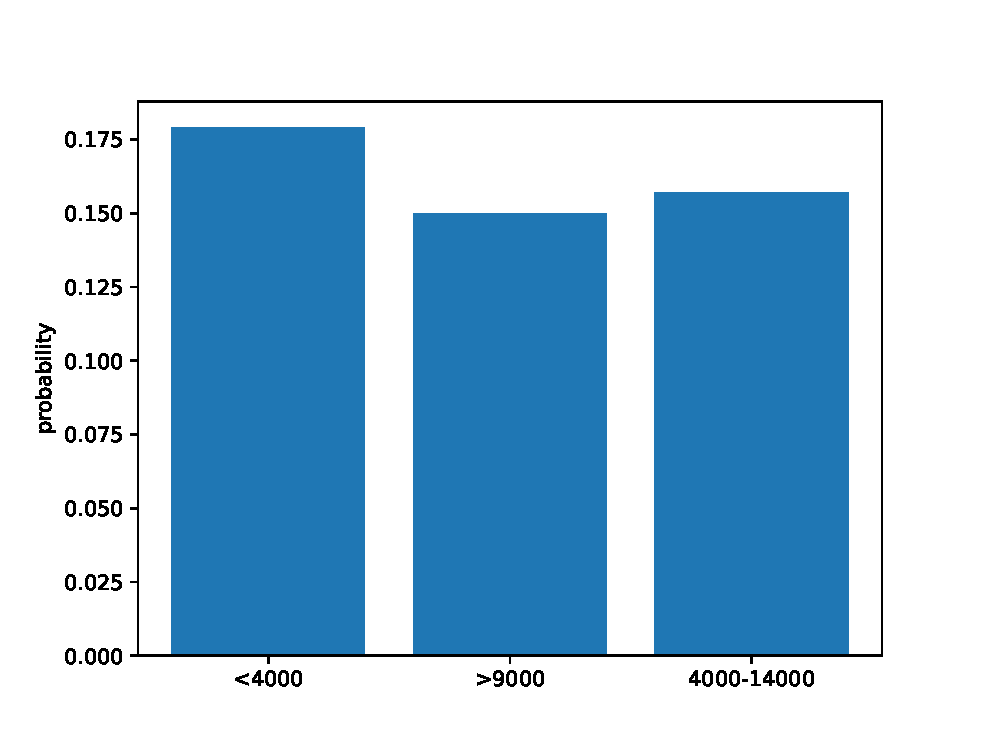
\includegraphics[width=\columnwidth]{./figures/probexm/probexm6.eps}
%	\caption{probability of distance covered by tyre }
%	\label{fig:bt6}
%	\begin{lstlisting}
%	figs/probexm/probexm6.eps
%	\end{lstlisting}
%\end{figure}
\end{enumerate}


\item The percentage of marks obtained by a student in the monthly unit tests are given in Table \ref{table:prob_exam7}
below.
Based on this data, find the probability that the student gets more than 70$\%$ marks in a unit test.\\

\begin{table}[!ht]
\centering
\resizebox{\columnwidth}{!}{
\begin{tabular}{ |c|c|c|c|c|c| } 
 \hline
 \textbf{Unit test} &I &II &III &IV &V \\ 
 \hline
 \textbf{Frequency }&69 &71 &73 &68 &74\\ 
 \hline
\end{tabular}
}
\caption{}
\label{table:prob_exam7}
\end{table}
\solution
From the given information,
\begin{align}
\pr{X>70} &= \frac{3}{5}
\\
&= 0.6
\end{align}

\item Consider the frequency distribution in Table \ref{table:prob_exam9} below which gives the weights of 38 students of a class.
(i) Find the probability that the weight of a student in the class lies in the interval 46-50 kg.\\
(ii) Give two events in this context, one having probability 0 and the other having probability 1.

%
\begin{table}[!ht]
\centering
\resizebox{\columnwidth}{!}{
\begin{tabular}{ |c|c| } 
 \hline
 \textbf{Weights (in kg)} &\textbf{Number of students }\\ 
 \hline
 31-35 &9\\
 36-40 &5\\
 41-45 &14\\
 46-50 &3\\
 51-55 &1\\
 56-60 &2\\
 61-65 &2\\
 66-70 &1\\
 71-75 &1\\
 \hline
 \textbf{Total} &38\\
 \hline
\end{tabular}
}
\caption{}
\label{table:prob_exam9}
\end{table}
\solution
\begin{enumerate}
\item 
From the given information, 
\begin{align}
\pr{46<X<50} &= \frac{3}{38}
\\
&= 0.079
\end{align}

\item There is no student whose weight is less than 31 kg thus the probability of a student to have the weight less than 31 kg = 0\\

All of the student in this context  have the weight between 31-75 so we can say that the probability of the students to have the weight in the range 31-75 = 1
\end{enumerate}

\item Fifty seeds were selected at random from each of 5 bags of seeds, and were kept under standardised conditions favourable to germination. After 20 days, the
number of seeds which had germinated in each collection were counted and recorded in Table \ref{table:prob_exam10}

What is the probability of germination of
(i)more than 40 seeds in a bag?\\
(ii) 49 seeds in a bag?\\
(iii) more that 35 seeds in a bag?\\

\begin{table}[!ht]
\centering
\resizebox{\columnwidth}{!}{
\begin{tabular}{ |c|c|c|c|c|c| } 
 \hline
 \textbf{Bag} &1 &2 &3 &4 &5\\ 
 \hline
\textbf{No.of seeds germinated} &40 &48 &42 &39 &41 \\ 
 \hline
\end{tabular}
}
\caption{}
\label{table:prob_exam10}
\end{table}
\solution
Let $X$ represent the seeds and $Y$ represent the bags.
\begin{enumerate}
\item 
\begin{align}
\pr{X > 40} &= \frac{3}{5}
\\
&= 0.6
\end{align}
\item
\begin{align}
\pr{X=49} &= \frac{0}{5}
\\
&= 0
\end{align}
\item 
\begin{align}
\pr{X>35} &= \frac{5}{5}
\\
&= 1
\end{align}
Related code is available in
\begin{lstlisting}
solutions/1-10/codes/probexm/probexm10.py
\end{lstlisting}
%\begin{figure}[!ht]
%	\centering
%	\includegraphics[width=\columnwidth]{./figures/probexm/probexm10.eps}
%	\caption{probability of germinated seeds in a bag }
%	\label{fig:bt10}
%	\begin{lstlisting}
%	figs/probexm/probexm10.eps
%	\end{lstlisting}
%\end{figure}
\end{enumerate}

    \item 1500 families with 2 children were selected randomly, and the following data in Table \ref{table:1.2.2} were recorded.
Compute the probability of a family, chosen at random, having
\begin{enumerate}
\item 2 girls
\item  1 girl
\item  No girl
\end{enumerate}
Also check whether the sum of these probabilities is 1.
\begin{table}[!ht]
\centering
\begin{tabular}{ |c|c|c|c| } 
 \hline
 \textbf{No.of girls in a family} &2 &1 &0\\ 
 \hline
 \textbf{No. of families}  &475 &814 &211\\ 
 \hline 
\end{tabular}
\caption{}
\label{table:1.2.2}
\end{table}
\\
\solution
In general, the complex number $\myvec{a_1\\a_2}$ has the matrix representation
\begin{align}
\label{eq:3.4.1_Complex}
\myvec{a_1\\a_2} &= \myvec{a_1 & -a_2\\ a_2 & a_1}\myvec{1\\0}
\\
&= \vec{T}_a\myvec{1\\0}
\\
\implies \myvec{5\\-3}&=\myvec{5&3\\-3&5}\myvec{1\\0}
\end{align}
Then,
\begin{align}
\myvec{5\\-3}^3 &\triangleq\myvec{5&3\\-3&5}^3\myvec{1\\0}
\\
 &= \myvec{-10&198\\-198&-10} \myvec{1\\0}
\\
&=\myvec{-10\\-198}
\end{align}
The python code for above problem is
\begin{lstlisting}
codes/line/comp.py
\end{lstlisting}


\item In a particular section of Class IX, 40 students were asked about the months of their birth and the following graph in Fig. \ref{fig:1.2.3}
was prepared for the data so obtained.     Find the probability that a student of the class was born in August.

\renewcommand{\theequation}{\theenumi}
\begin{enumerate}[label=\arabic*.,ref=\thesubsection.\theenumi]
\numberwithin{equation}{enumi}
\item Refer the table below\\

\begin{tabular}{ cccccccccc} 
	
	5 &3 &10 &20 &25 &11 &13 &7 &12 &31\\
	19 &10 &12 &17 &18 &11 &32 &17 &16 &2\\
	7 &9 &7 &8 &3 &5 &12 &15 &18 &3 \\
	12 &14 &2 &9 &6 &15 &15 &7 &6 &12\\ 
\end{tabular}\\

What is the empirical probability that an engineer lives:\\
(i) less than 7 km from her place of work?\\
(ii)more than or equal to 7 km from her place of work?\\
(iii) within $\frac{1}{2}$km from her place of work?\\

\end{enumerate}    
\solution
In general, the complex number $\myvec{a_1\\a_2}$ has the matrix representation
\begin{align}
\label{eq:3.4.1_Complex}
\myvec{a_1\\a_2} &= \myvec{a_1 & -a_2\\ a_2 & a_1}\myvec{1\\0}
\\
&= \vec{T}_a\myvec{1\\0}
\\
\implies \myvec{5\\-3}&=\myvec{5&3\\-3&5}\myvec{1\\0}
\end{align}
Then,
\begin{align}
\myvec{5\\-3}^3 &\triangleq\myvec{5&3\\-3&5}^3\myvec{1\\0}
\\
 &= \myvec{-10&198\\-198&-10} \myvec{1\\0}
\\
&=\myvec{-10\\-198}
\end{align}
The python code for above problem is
\begin{lstlisting}
codes/line/comp.py
\end{lstlisting}


\item Three coins are tossed simultaneously 200 times with the following frequencies of different outcomeslisted in Table \ref{table:1.2.4}.
If the three coins are simultaneously tossed again, compute the probability of 2 heads coming up.
%
\begin{table}[!ht]
%\resizebox{\columnwidth}{20pt}{%
\resizebox{\columnwidth}{!}{%
\begin{tabular}{ |c|c|c|c|c| } 
 \hline
 \textbf{Outcome} &3 heads &2 heads &1 head &No head\\ 
 \hline
 \textbf{Frequency}  &23 &72 &77 &28\\ 
 \hline
\end{tabular}%\\
}
\caption{}
\label{table:1.2.4}
\end{table}
\\
\solution
In general, the complex number $\myvec{a_1\\a_2}$ has the matrix representation
\begin{align}
\label{eq:3.4.1_Complex}
\myvec{a_1\\a_2} &= \myvec{a_1 & -a_2\\ a_2 & a_1}\myvec{1\\0}
\\
&= \vec{T}_a\myvec{1\\0}
\\
\implies \myvec{5\\-3}&=\myvec{5&3\\-3&5}\myvec{1\\0}
\end{align}
Then,
\begin{align}
\myvec{5\\-3}^3 &\triangleq\myvec{5&3\\-3&5}^3\myvec{1\\0}
\\
 &= \myvec{-10&198\\-198&-10} \myvec{1\\0}
\\
&=\myvec{-10\\-198}
\end{align}
The python code for above problem is
\begin{lstlisting}
codes/line/comp.py
\end{lstlisting}

\item Refer to Table \ref{table:1.2.5}.
\begin{enumerate}
\item  Find the probability that a student obtained less than 20$\%$ in the mathematics test.
\item  Find the probability that a student obtained marks 60 or above.
\end{enumerate}
\begin{table}[!ht]
\centering
\begin{tabular}{ |c|c| } 
 \hline
 \textbf{Marks} &\textbf{Number of students}\\
 \hline
  0-20 &7\\ 
  20-30 &10\\ 
  30-40 &10\\ 
  40-50 &20\\ 
  50-60 &20\\ 
  60-70 &15\\ 
  70-above &8\\ 
  \hline
 \textbf{Total}  &90\\ 
 \hline
\end{tabular}
\caption{}
\label{table:1.2.5}
\end{table}
\solution
In general, the complex number $\myvec{a_1\\a_2}$ has the matrix representation
\begin{align}
\label{eq:3.4.1_Complex}
\myvec{a_1\\a_2} &= \myvec{a_1 & -a_2\\ a_2 & a_1}\myvec{1\\0}
\\
&= \vec{T}_a\myvec{1\\0}
\\
\implies \myvec{5\\-3}&=\myvec{5&3\\-3&5}\myvec{1\\0}
\end{align}
Then,
\begin{align}
\myvec{5\\-3}^3 &\triangleq\myvec{5&3\\-3&5}^3\myvec{1\\0}
\\
 &= \myvec{-10&198\\-198&-10} \myvec{1\\0}
\\
&=\myvec{-10\\-198}
\end{align}
The python code for above problem is
\begin{lstlisting}
codes/line/comp.py
\end{lstlisting}

\item The distance (in kms) of 40 engineers from their residence to their place of work were found as follows in Table \ref{table:1.2.7}.
What is the empirical probability that an engineer lives
\begin{enumerate}
\item less than 7 km from her place of work?
\item more than or equal to 7 km from her place of work? 
\item within $\frac{1}{2}$km from her place of work?
\end{enumerate}

\begin{table}[!ht]
\centering
\begin{tabular}{ cccccccccc} 

 5 &3 &10 &20 &25 &11 &13 &7 &12 &31\\
 19 &10 &12 &17 &18 &11 &32 &17 &16 &2\\
 7 &9 &7 &8 &3 &5 &12 &15 &18 &3 \\
 12 &14 &2 &9 &6 &15 &15 &7 &6 &12\\ 
 \end{tabular}\\
\caption{}
\label{table:1.2.7}
\end{table}
\solution
In general, the complex number $\myvec{a_1\\a_2}$ has the matrix representation
\begin{align}
\label{eq:3.4.1_Complex}
\myvec{a_1\\a_2} &= \myvec{a_1 & -a_2\\ a_2 & a_1}\myvec{1\\0}
\\
&= \vec{T}_a\myvec{1\\0}
\\
\implies \myvec{5\\-3}&=\myvec{5&3\\-3&5}\myvec{1\\0}
\end{align}
Then,
\begin{align}
\myvec{5\\-3}^3 &\triangleq\myvec{5&3\\-3&5}^3\myvec{1\\0}
\\
 &= \myvec{-10&198\\-198&-10} \myvec{1\\0}
\\
&=\myvec{-10\\-198}
\end{align}
The python code for above problem is
\begin{lstlisting}
codes/line/comp.py
\end{lstlisting}



\item An organisation selected 2400 families at random and surveyed them to determine a relationship between income level and the number of vehicles in a family. The information gathered is listed in the Table \ref{table:1.2.8}
Suppose a family is chosen. Find the probability that the family chosen is
\begin{enumerate}
\item  earning \rupee 10000 – \rupee 13000 per month and owning exactly 2 vehicles.
\item  earning \rupee 16000 or more per month and owning exactly 1 vehicle.
\item  earning less than \rupee 7000 per month and does not own any vehicle.
\item  earning \rupee 13000 – \rupee 16000 per month and owning more than 2 vehicles.
\item owning not more than 1 vehicle.
\end{enumerate}
%
\begin{table}[!ht]
\centering
\begin{tabular}{|c|c|c|c|c|}
\hline
\textbf{Monthly income} &\multicolumn{4}{c|}{\textbf{vehicles per family }}\\
\cline{2-5}
(in \textbf{\rupee}) &\textbf{0} &\textbf{1} &\textbf{2} &\textbf{Above 2}\\
\hline
Less than 7000 &10 &160 &25 &0\\
\hline
7000-10000 &0 &305 &27 &2\\
\hline
10000-13000 &1 &535 &29 &1\\
\hline
13000-16000 &2 &469 &59 &25\\
\hline
16000 or more  &1 &579 &82 &88 \\
\hline
\end{tabular}
\caption{}
\label{table:1.2.8}
\end{table}
\solution
In general, the complex number $\myvec{a_1\\a_2}$ has the matrix representation
\begin{align}
\label{eq:3.4.1_Complex}
\myvec{a_1\\a_2} &= \myvec{a_1 & -a_2\\ a_2 & a_1}\myvec{1\\0}
\\
&= \vec{T}_a\myvec{1\\0}
\\
\implies \myvec{5\\-3}&=\myvec{5&3\\-3&5}\myvec{1\\0}
\end{align}
Then,
\begin{align}
\myvec{5\\-3}^3 &\triangleq\myvec{5&3\\-3&5}^3\myvec{1\\0}
\\
 &= \myvec{-10&198\\-198&-10} \myvec{1\\0}
\\
&=\myvec{-10\\-198}
\end{align}
The python code for above problem is
\begin{lstlisting}
codes/line/comp.py
\end{lstlisting}


\item Eleven bags of wheat flour, each marked 5 kg, actually contained the following weights of flour (in kg)\\
4.97 5.05 5.08 5.03 5.00 5.06 5.08 4.98 5.04 5.07 5.00\\
Find the probability that any of these bags chosen at random contains more than 5 kg of flour.\\
\solution
%In general, the complex number $\myvec{a_1\\a_2}$ has the matrix representation
\begin{align}
\label{eq:3.4.1_Complex}
\myvec{a_1\\a_2} &= \myvec{a_1 & -a_2\\ a_2 & a_1}\myvec{1\\0}
\\
&= \vec{T}_a\myvec{1\\0}
\\
\implies \myvec{5\\-3}&=\myvec{5&3\\-3&5}\myvec{1\\0}
\end{align}
Then,
\begin{align}
\myvec{5\\-3}^3 &\triangleq\myvec{5&3\\-3&5}^3\myvec{1\\0}
\\
 &= \myvec{-10&198\\-198&-10} \myvec{1\\0}
\\
&=\myvec{-10\\-198}
\end{align}
The python code for above problem is
\begin{lstlisting}
codes/line/comp.py
\end{lstlisting}


\item From Table \ref{table:1.2.10}, 
prepare a frequency distribution table, regarding the concentration of sulphur dioxide in the air in parts per million of a certain city for 30 days.   Using this table, find the probability of the concentration of sulphur dioxide in the interval 0.12 - 0.16 on any of these days.
%
\begin{table}[!ht]
\centering
\begin{tabular}{ cccccc} 

  0.03 &0.08 &0.08 &0.09 &0.04 &0.17 \\
 0.16 &0.05 &0.02 &0.06 &0.18 &0.20 \\
 0.11 &0.08 &0.12 &0.13 &0.22 &0.07  \\
 0.08 &0.01 &0.10 &0.06 &0.09 &0.18 \\ 
  0.11 &0.07 &0.05 &0.07 &0.01 &10.04 \\ 
 \end{tabular}\\
\caption{}
\label{table:1.2.10}
\end{table}
\solution
In general, the complex number $\myvec{a_1\\a_2}$ has the matrix representation
\begin{align}
\label{eq:3.4.1_Complex}
\myvec{a_1\\a_2} &= \myvec{a_1 & -a_2\\ a_2 & a_1}\myvec{1\\0}
\\
&= \vec{T}_a\myvec{1\\0}
\\
\implies \myvec{5\\-3}&=\myvec{5&3\\-3&5}\myvec{1\\0}
\end{align}
Then,
\begin{align}
\myvec{5\\-3}^3 &\triangleq\myvec{5&3\\-3&5}^3\myvec{1\\0}
\\
 &= \myvec{-10&198\\-198&-10} \myvec{1\\0}
\\
&=\myvec{-10\\-198}
\end{align}
The python code for above problem is
\begin{lstlisting}
codes/line/comp.py
\end{lstlisting}

\item  
A, B, O, O, AB, O, A, O, B, A, O, B, A, O,\\ O,
A, AB, O, A, A, O, O, AB, B, A, O, B, A, B, O.\\
prepare a frequency distribution table regarding the blood groups of 30 students of a class. Use this table to determine the probability that a student of this class, selected at random, has blood group AB.\\
\item Determine P(E/F), if mother, father and son line up at random for a family picture\\
E : son on one end, F : father in middle\\
\item Consider the experiment of throwing a die, if a multiple of 3 comes up, throw the die again and if any other number comes, toss a coin. Find the conditional probability of the event 'the coin shows a tail', given that 'at least one die shows a 3'.\\
\solution
Let $X \in {1,2}$ represent the Bag  and $Y \in \cbrak{0,1}$ represent the colour, where 1 denotes red.  From the given information,
\begin{align}
\pr{X=1}&=\pr{X=2} = \frac{1}{2}
\\
\pr{Y = 1|X=1} &= \frac{3}{7}
\\
\pr{Y = 1|X=2} &= \frac{5}{11}
\end{align}
Thus,
{\tiny
\begin{align}
\pr{X=2|Y=1} &= \frac{\pr{X=2,Y=1}}{\pr{Y=1}}
\\
&=\frac{\pr{Y=1|X=2}\pr{X=2}}{\pr{Y=1|X=1}\pr{X=1}+\pr{Y=1|X=2}\pr{X=2}}
\\
&=\frac{\frac{5}{11}\times \frac{1}{2}}{\frac{3}{7}\times \frac{1}{2}+\frac{5}{11}\times \frac{1}{2}}
\\
&=\frac{35}{68}
\end{align}
}

\item One card is drawn from a well-shuffled deck of 52 cards. Find the probability of getting
(i) a king of red colour\\
(ii) a face card\\
(iii) a red face card\\
(iv) the jack of hearts \\
(v) a spade \\
(vi) the queen of diamonds
\\
\solution
In general, the complex number $\myvec{a_1\\a_2}$ has the matrix representation
\begin{align}
\label{eq:3.4.1_Complex}
\myvec{a_1\\a_2} &= \myvec{a_1 & -a_2\\ a_2 & a_1}\myvec{1\\0}
\\
&= \vec{T}_a\myvec{1\\0}
\\
\implies \myvec{5\\-3}&=\myvec{5&3\\-3&5}\myvec{1\\0}
\end{align}
Then,
\begin{align}
\myvec{5\\-3}^3 &\triangleq\myvec{5&3\\-3&5}^3\myvec{1\\0}
\\
 &= \myvec{-10&198\\-198&-10} \myvec{1\\0}
\\
&=\myvec{-10\\-198}
\end{align}
The python code for above problem is
\begin{lstlisting}
codes/line/comp.py
\end{lstlisting}

\item Five cards—the ten, jack, queen, king and ace of diamonds, are well-shuffled with their
face downwards. One card is then picked up at random.\\
(i) What is the probability that the card is the queen?\\
(ii) If the queen is drawn and put aside, what is the probability that the second card
picked up is (a) an ace? (b) a queen?
\\
\solution
In general, the complex number $\myvec{a_1\\a_2}$ has the matrix representation
\begin{align}
\label{eq:3.4.1_Complex}
\myvec{a_1\\a_2} &= \myvec{a_1 & -a_2\\ a_2 & a_1}\myvec{1\\0}
\\
&= \vec{T}_a\myvec{1\\0}
\\
\implies \myvec{5\\-3}&=\myvec{5&3\\-3&5}\myvec{1\\0}
\end{align}
Then,
\begin{align}
\myvec{5\\-3}^3 &\triangleq\myvec{5&3\\-3&5}^3\myvec{1\\0}
\\
 &= \myvec{-10&198\\-198&-10} \myvec{1\\0}
\\
&=\myvec{-10\\-198}
\end{align}
The python code for above problem is
\begin{lstlisting}
codes/line/comp.py
\end{lstlisting}

\item A box contains 90 discs which are numbered from 1 to 90. If one disc is drawn at random
from the box, find the probability that it bears (i) a two-digit number (ii) a perfect
square number (iii) a number divisible by 5.
\\
\solution
In general, the complex number $\myvec{a_1\\a_2}$ has the matrix representation
\begin{align}
\label{eq:3.4.1_Complex}
\myvec{a_1\\a_2} &= \myvec{a_1 & -a_2\\ a_2 & a_1}\myvec{1\\0}
\\
&= \vec{T}_a\myvec{1\\0}
\\
\implies \myvec{5\\-3}&=\myvec{5&3\\-3&5}\myvec{1\\0}
\end{align}
Then,
\begin{align}
\myvec{5\\-3}^3 &\triangleq\myvec{5&3\\-3&5}^3\myvec{1\\0}
\\
 &= \myvec{-10&198\\-198&-10} \myvec{1\\0}
\\
&=\myvec{-10\\-198}
\end{align}
The python code for above problem is
\begin{lstlisting}
codes/line/comp.py
\end{lstlisting}

\item A child has a die whose six faces show the letters as given in Fig. \ref{fig:130_dice}	.

\begin{figure}[!ht]
\centering
\resizebox{\columnwidth}{!}{%A child has a die whose six faces show the letters as given below:\\

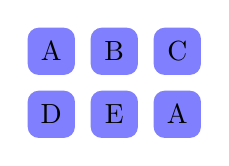
\begin{tikzpicture}[outer sep=0.05cm,node distance=0.8cm,]
\tikzstyle{bigbox} = [draw=white!50, thick, fill=white!10, rounded corners, rectangle]
\tikzstyle{box} = [minimum size=0.6cm, rounded corners,rectangle, fill=blue!50]
%
\node[box] (11) {A};
\node[box,right of=11] (12) {B};
\node[box,right of=12] (13) {C};
\node[box,below of=11] (21) {D};
\node[box,right of=21] (22) {E};
\node[box,right of=22] (23) {A};
\end{tikzpicture}
%\\
%The die is thrown once. What is the probability of getting (i) A? (ii) D?
}
%\resizebox{\columnwidth}{!}{
\begin{tikzpicture}

\draw (0,0) node[anchor=north]{$B$}
  -- (4,8) node[anchor=west]{$A$}
  -- (8,0) node[anchor=north]{$C$}
  -- cycle;
\draw (4,0) node[anchor=north]{$E$}
  -- (2,4) node[anchor=east]{$D$}
  -- (6,4) node[anchor=west]{$F$}
  -- cycle;
\end{tikzpicture}

}
\caption{}
\label{fig:130_dice}	
\end{figure}

The die is thrown once. What is the probability of getting (i) A? (ii) D?
\\
\solution
In general, the complex number $\myvec{a_1\\a_2}$ has the matrix representation
\begin{align}
\label{eq:3.4.1_Complex}
\myvec{a_1\\a_2} &= \myvec{a_1 & -a_2\\ a_2 & a_1}\myvec{1\\0}
\\
&= \vec{T}_a\myvec{1\\0}
\\
\implies \myvec{5\\-3}&=\myvec{5&3\\-3&5}\myvec{1\\0}
\end{align}
Then,
\begin{align}
\myvec{5\\-3}^3 &\triangleq\myvec{5&3\\-3&5}^3\myvec{1\\0}
\\
 &= \myvec{-10&198\\-198&-10} \myvec{1\\0}
\\
&=\myvec{-10\\-198}
\end{align}
The python code for above problem is
\begin{lstlisting}
codes/line/comp.py
\end{lstlisting}

\item Which of the following arguments are correct and which are not correct? Give reasons
for your answer.\\
(i) If two coins are tossed simultaneously there are three possible outcomes—two
heads, two tails or one of each. Therefore, for each of these outcomes, the
probability is $\frac{1}{3}$ \\
(ii) If a die is thrown, there are two possible outcomes—an odd number or an even
number. Therefore, the probability of getting an odd number is $\frac{1}{2}$.
\\
\solution
\renewcommand{\theequation}{\theenumi}
\begin{enumerate}[label=\arabic*.,ref=\thesubsubsection.\theenumi]
\numberwithin{equation}{enumi}
\item In the given question,
\\
The sample size = Total number of possibilities(S)=6
\begin{align}
\myvec{1&2&3&4&5&6}
\end{align}
Event size= Odd number =3
\begin{align}
\myvec{1&3&5}
\end{align}
Probability for this event is = $\frac{1}{2}$
\\
The python code for the distribution of data,
\begin{lstlisting}
prob/codes/prob6_b.py
\end{lstlisting}
This shows the diagrametic representation of dice with the live update of probability with the role of dice.
\end{enumerate}

\item Two customers Shyam and Ekta are visiting a particular shop in the same week (Tuesday
to Saturday). Each is equally likely to visit the shop on any day as on another day. What
is the probability that both will visit the shop on\\
(i) the same day?\\
(ii) consecutive days?\\
(iii) different days?
\\
\solution
In general, the complex number $\myvec{a_1\\a_2}$ has the matrix representation
\begin{align}
\label{eq:3.4.1_Complex}
\myvec{a_1\\a_2} &= \myvec{a_1 & -a_2\\ a_2 & a_1}\myvec{1\\0}
\\
&= \vec{T}_a\myvec{1\\0}
\\
\implies \myvec{5\\-3}&=\myvec{5&3\\-3&5}\myvec{1\\0}
\end{align}
Then,
\begin{align}
\myvec{5\\-3}^3 &\triangleq\myvec{5&3\\-3&5}^3\myvec{1\\0}
\\
 &= \myvec{-10&198\\-198&-10} \myvec{1\\0}
\\
&=\myvec{-10\\-198}
\end{align}
The python code for above problem is
\begin{lstlisting}
codes/line/comp.py
\end{lstlisting}

\item A die is numbered in such a way that its faces show the numbers 1, 2, 2, 3, 3, 6. It is thrown two times and the total score in two throws is noted. Complete the following
table which gives a few values of the total score on the two throws:
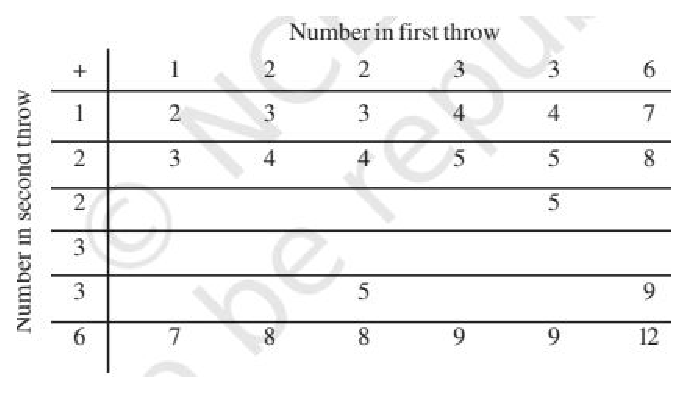
\includegraphics[width=\columnwidth]{./prob/figs/rows.eps}\\
What is the probability that the total score is
(i) even? (ii) 6? (iii) at least 6?
\\
\solution
In general, the complex number $\myvec{a_1\\a_2}$ has the matrix representation
\begin{align}
\label{eq:3.4.1_Complex}
\myvec{a_1\\a_2} &= \myvec{a_1 & -a_2\\ a_2 & a_1}\myvec{1\\0}
\\
&= \vec{T}_a\myvec{1\\0}
\\
\implies \myvec{5\\-3}&=\myvec{5&3\\-3&5}\myvec{1\\0}
\end{align}
Then,
\begin{align}
\myvec{5\\-3}^3 &\triangleq\myvec{5&3\\-3&5}^3\myvec{1\\0}
\\
 &= \myvec{-10&198\\-198&-10} \myvec{1\\0}
\\
&=\myvec{-10\\-198}
\end{align}
The python code for above problem is
\begin{lstlisting}
codes/line/comp.py
\end{lstlisting}


\end{enumerate}

